%%
%% 2019 07 04 Ph. G. Freimann
%%

\section{Funktionen}\index{Funktion|textbf}
\sectuntertitel{longitudo, latitudo (Begriffe nach Nikolaus von Oresme)}
%%%%%%%%%%%%%%%%%%%%%%%%%%%%%%%%%%%%%%%%%%%%%%%%%%%%%%%%%%%%%%%%%%%%%%%%%%%%%%%%%
\subsection*{Lernziele}

\begin{itemize}
 \item Zuordnung
 \item Mengenbegriffe: Definitionsmenge\index{Definitionsmenge} (= Definitionsbereich\index{Definitionsbereich}) vs. Quellbereich\index{Quellbereich}
 \item Wertebereich (= Bildmenge) vs. Zielmenge\index{Zielmenge}
   (=Zielmenge\index{Zielmenge} oder Wertevorrat\index{Wertevorrat})
 \item Darstellungsarten
   \begin{itemize}
      \item Wertetabelle
      \item Graphen\index{Graph}
      \item Funktionsterm
   \end{itemize}
 \item verschiedene Notationen
 \item Gleichungen visualisieren
 \item Achsen\index{Achse}
 \item Funktionsgleichung
 \item Abhängige, unabhängige Variable / Argument, Parameter, Funktionswert
\end{itemize}

\TALS{(\cite{frommenwiler17alg} S.161 (Kap. 3))}
\GESO{(\cite{marthaler17}       S.211 (Kap. 13))}

\newpage
\subsection{Allgemeiner Funktionsbegriff}\index{Funktion!allgemeiner Begriff}


\begin{definition}{Funktion}{}
    Eine \textbf{Funktion}\index{Funktion} ist eine \textbf{Zuordnung}\index{Zuordnung}, die jeder Zahl
    $x$ aus einer Definitionsmenge \textbf{genau} eine Zahl $y$ aus
    einer Zielmenge\index{Zielmenge} zuordnet.\\
\end{definition}
    
Die Menge aller getroffenen Werte aus der Zielmenge wird \textbf{Wertebereich}\index{Wertebereich}
(oder Bildmenge) genannt.\GESO{ Achtung im Buch \cite{marthaler17} wird
  mit dem Begriff «Bildmenge» der Wertevorrat bezeichnet!}

Mengenbezeichnungen bei Gleichungen (Diese Mengen sind bereits
bekannt\footnote{Die Definitionsmenge bezeichnet hier die Menge aller
  Zahlen für die alle Terme definiert sind.}):

\begin{tabular}{cp{4cm}l}

  \raisebox{-3cm}{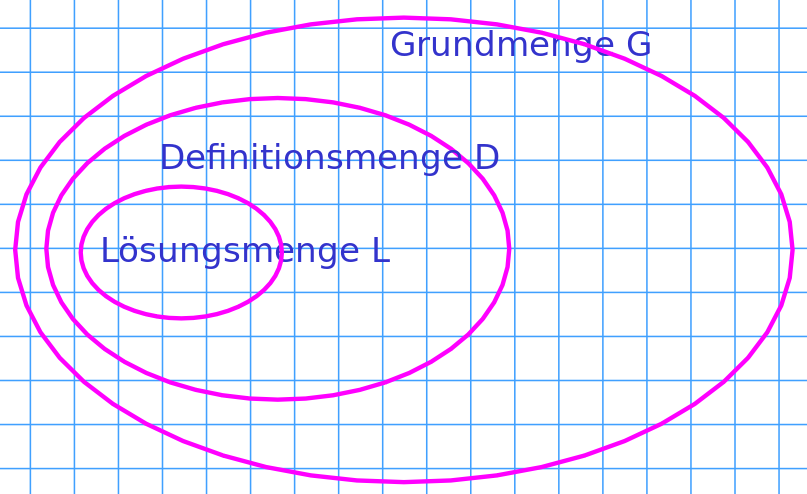
\includegraphics[width=8cm]{allg/funktionen/img/MengenbezeichnungenBeiGleichungen.png}}
  & Beispiel & \makecell{$\frac{1}{x-3}=5$\\
  $\mathbb{G}=\mathbb{R}$\\
  $\mathbb{D}=\mathbb{R}\backslash{}\{3\}$\\
  $\mathbb{L}_x = 3.2$}
\end{tabular}

\vspace{6mm}
Mengenbezeichnungen bei Funktionen:
\TRAINER{\begin{center}
  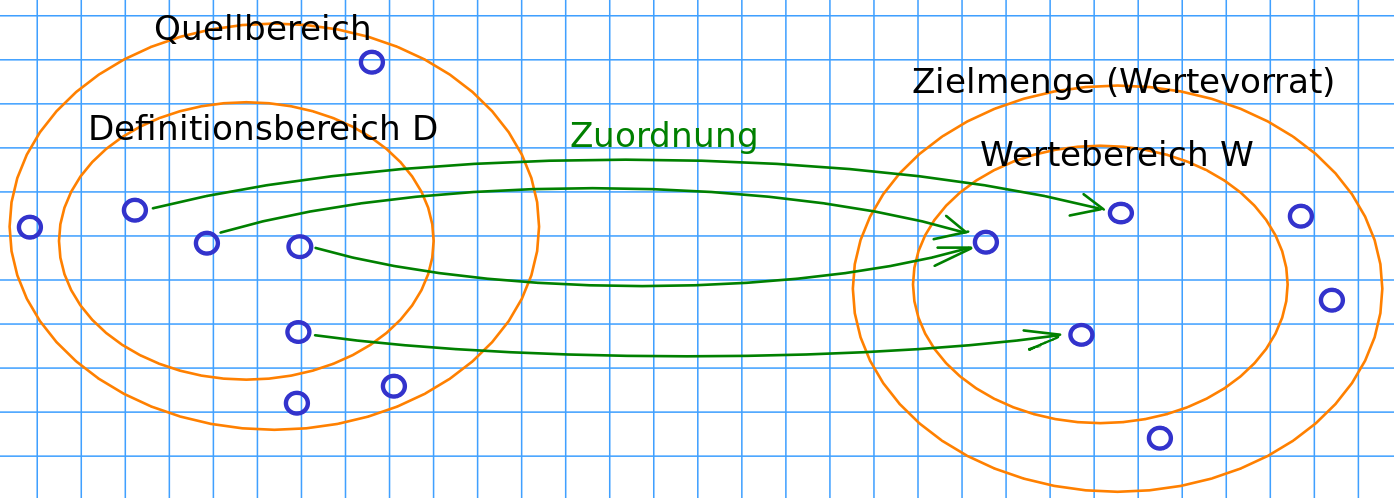
\includegraphics[width=16cm]{allg/funktionen/img/MengenbezeichnungenBeiFunktionen.png}
\end{center}
}%% END TRAINER

\noTRAINER{\begin{center}
  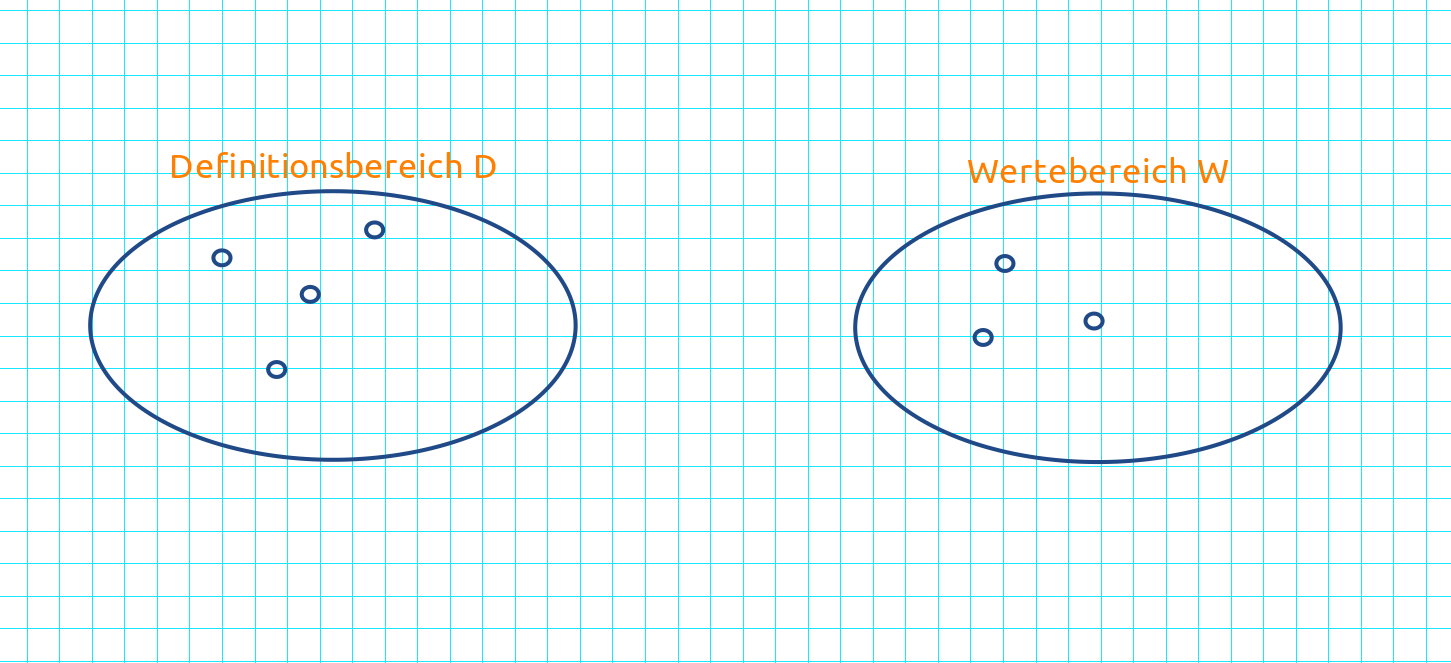
\includegraphics[width=16cm]{allg/funktionen/img/MengenbezeichnungenBeiFunktionenLeer.png}
\end{center}
}%% END no TRAINER

\TALS{
\begin{beispiel}{reelle Funktion}{}
  Funktion Sinus $\sin()$:
  $\mathbb{D} = \mathbb{R}$; $\mathbb{W}= [-1; 1]$
  $$\sin: \mathbb{R} \rightarrow [-1; 1] \textrm{ mit } \varphi\mapsto{}\sin(\varphi) $$
\end{beispiel}

\begin{beispiel}{}{}
  Funktion Tangens $\tan()$:
  $\mathbb{D} = \mathbb{R}\backslash\{\pm{}90^\circ, \pm{}270^\circ, \pm{}450^\circ, ...\}$; $\mathbb{W}= \mathbb{R}$
    
  $$\tan: \mathbb{R}\backslash\{90^\circ{}+z\cdot{}180^\circ{}|z \in \mathbb{Z}\} \rightarrow \mathbb{R} \textrm{ mit } \alpha\mapsto{}\tan(\alpha) $$
\end{beispiel}
}

\begin{bemerkung}{}{}
  Zum Wertebereich: Wo der Begriff Quellbereich (eine theoretische Obermenge
  des Definitionsbereichs\index{Definitionsbereich}) kaum praktische Bedeutung hat,
  wird jedoch in speziellen Fällen statt dem Wertebereich die
  \textbf{Zielmenge}\index{Zielmenge}\footnote{Die Zielmenge
    wird auch Zielbereich, Wertevorrat\index{Wertevorrat},
    Cobereich\index{Cobereich} oder Nachbereich\index{Nachbereich}
    genannt (\cite{FormelnUndTafeln19}).}
  angegeben; meist daher, weil der
  Wertebereich in komplexen, fraktalen, sprungstetigen oder sonstwie komplizierten Funktionen schlicht
  und ergreifend nicht bekannt ist.\footnote{\textbf{Beispiel 1}: Bei der Funktion
    «mittlere Tagestemperatur» ist zwar die Zielmenge ($\mathbb{R}[{}^\circ]$)
    bekannt, jedoch sind die effektiv getroffenen Bildwerte meist nur
    zwischen $-40^\circ$ und $+50^\circ$ vorzufinden (daher ist der
    effektiv eintretende Wertebereich erst dann bekannt, wenn das Wetter
    bereits eingetreten ist bzw. auch gemessen wurde). \\
    \textbf{Beispiel 2}: (Sei $\pi$ die Kreiszahl.) Der Funktion $f: n\mapsto f(n)$; $\mathbb{N} \rightarrow \{0, 1, 2, 3, ..., 9\} \textrm{mit} f(n) = $
    «millionste Nachkommastelle von $n\pi$»
    kann der effektive Wertebereich nicht
  angesehen werden, bevor wir genügend oft die millionste Ziffer von
  $n\pi$ berechnet haben. Hier ist vorerst nur die Zielmenge, nicht
  aber der Wertebereich bekannt.}
\end{bemerkung}


\GESO{
  \begin{beispiel}{Jahreszins}{}
    Jahreszins bei gegebenem Jahreszinssatz von 3\%:

    $\mathbb{D} = \mathbb{R}^{+}$; $\mathbb{W} = \mathbb{R}^{+}$

    $\textrm{Zins}: \mathbb{R}^{+} \rightarrow \mathbb{R}^{+} \textrm{ mit } k \mapsto{} k\cdot{}\frac{3}{100}$
    \end{beispiel}
}

\GESOAadB{232}{20., 21. und 22.}

\newpage


\subsection{Arten der Darstellung}
\begin{itemize}
\item Wertetabelle\index{Wertetabelle}:

  \begin{tabular}{c|cccccc}$x$ & -2 & -1 & 0 & 1 & 2 & 2.5\\
    \hline
    $f(x)=y=x^2-1$ & \LoesungsRaumKurz{3} & \LoesungsRaumKurz{0} & \LoesungsRaumKurz{-1} & \LoesungsRaumKurz{0} & \LoesungsRaumKurz{3} & \LoesungsRaumKurz{5.25}\\ 
\end{tabular}
\item Graphen im rechtwinkligen Koordinatensystem
  
\noTRAINER{\bbwGraph{-3}{4}{-1.5}{6}{}}
\TRAINER{  \bbwFunction{-3}{4}{-1.5}{6}{\x*\x - 1 }{-2:2.5}}

\item Funktionsschreibweise\\
  $f: \mathbb{D} \rightarrow \mathbb{W}$\\
  Beispiel:\\
  $y=f(x)$ \zB $y=x^2-1$\\
  $f: x\mapsto y$ mit $x \in \mathbb{D}$ und $y \in \mathbb{W}$\\
  Alternative Notation: $f: x\mapsto{} f(x)$ oder $x\mapsto x^2-1$\\


  \subsubsection*{Notationen}

  \begin{tabular}{l|l}
    \textit{Begriff} & \textit{Beispiel(e)}\\\hline
    \textbf{Funktionsparameter}\index{Funktion!Parameter}\index{Parameter!Funktionen} & \TRAINER{$x$}\noTRAINER{\,\,\,\,\,\,\,\,\,\,\,\,\,\,\,\,\,\,\,\,\,\,\,\,\,\,\,\,\,\,\,\,\,\,\,\,\,\,\,\,\,\,\,\,\,\,\,\,\,\,\,}\\\hline
    \textbf{Funktionsargumente}\index{Funktion!Argument}\index{Argument!Funktionen}   & \TRAINER{Zahlen -2, -1, 0, 1, ...}\\\hline
    \textbf{Funktionswert}     \index{Funktion!Wert}\index{Wert!einer Funktion}       & \TRAINER{Wert von $x^2+1=y=f(x)$}\\\hline
    \textbf{Funktionsgleichung}\index{Funktion!Gleichung}\index{Gleichung!Funktion}   & \TRAINER{$y=x^2-1$ bzw. $y=f(x)$}\\\hline
  \end{tabular}

\end{itemize}
\newpage

\subsection*{Aufgaben}

\TALSAadB{165ff}{577. e) f) 578. b) 579. a) c) 580. a) c) 581.b)
  582. 587. 588. 592.}
\GESOAadB{231ff}{17. a) b) und f) und  19. a) b) e) und f)}
\newpage
